\documentclass[handout]{beamer} %
%\documentclass[11 pt]{beamer} %
\usepackage{verbatim}
\usepackage{graphicx}

\renewcommand{\thefootnote}{}	% Empty footnote style

\usefonttheme{serif}
\usetheme{Madrid} % My favorite!
\usecolortheme{seahorse} % Simple and clean template
\setbeamertemplate{navigation symbols}{}%remove navigation symbols
\setbeamertemplate{footline}[frame number]{}

\newcommand{\beginbackup}{
   \newcounter{framenumbervorappendix}
   \setcounter{framenumbervorappendix}{\value{framenumber}}
}
\newcommand{\backupend}{
   \addtocounter{framenumbervorappendix}{-\value{framenumber}}
   \addtocounter{framenumber}{\value{framenumbervorappendix}} 
}

\AtBeginSection[] 
{ 
  \begin{frame}[plain]{Outline} 
    \tableofcontents[currentsection] 
    \addtocounter{framenumber}{-1} 
  \end{frame} 
}

\usepackage{pgfpages}


\mode<handout>{
  \usetheme{default}
  \setbeamercolor{background canvas}{bg=black!5}
  \pgfpagesuselayout{4 on 1}[letterpaper,landscape,border shrink=2.5mm]
  \AtBeginSection[]{}
}


\usepackage{tikz}
\usetikzlibrary{shapes}
\tikzstyle{vertex}=[circle,fill=black!25,minimum size=10pt,inner sep=2pt]
\tikzstyle{Nvertex}=[circle,fill=white!25,minimum size=10pt,inner sep=2pt]
\tikzstyle{LabelStyle}=[fill=white,sloped]

\tikzstyle{big_vertex}=[circle,fill=red!15,minimum size=50pt,inner sep=2pt,draw=black!50]
\tikzstyle{med_vertex}=[circle,fill=red!10,minimum size=35pt,inner sep=2pt,draw=black!50]

\tikzstyle{macrostate_vertex}=[inner sep=3pt,draw=black!70]


\newcommand{\vertexshiftamount}{2.5}
\newcommand{\tikzpicscale}{1.5}

\newcommand{\TIKZenergylevel}{

  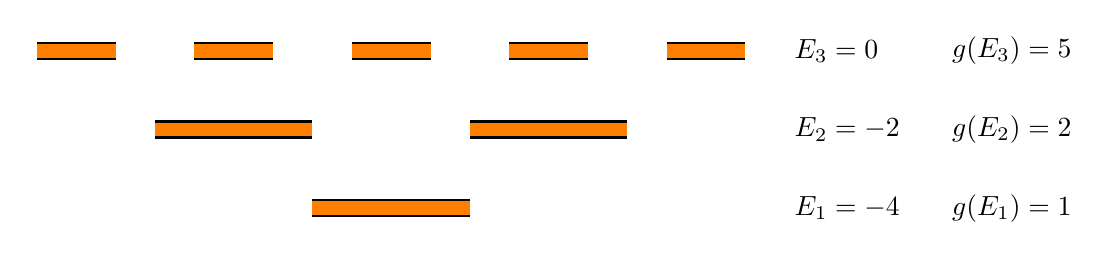
\begin{tikzpicture}
    \tikzset{level/.style   = {thick,
        double          = orange,
        double distance = 5pt}}
    
    \def\Espace{9};
    \def\Gspace{11};
    
    % Draw the energy levels.
    \draw[level] (3,0)  -- (5,0) node[right]{};
    \draw[] (\Espace,0) node[right] {$E_1=-4$};
    \draw[] (\Gspace,0) node[right] {$g(E_1)=1$};
    
    \draw[level] (1,1) -- (3,1) node[right] {};
    \draw[level] (5,1) -- (7,1) node[right] {};
    \draw[] (\Espace,1) node[right] {$E_2=-2$};
    \draw[] (\Gspace,1) node[right] {$g(E_2)=2$};
    
    \def\v{.5}; 
    \draw[level] (-1+\v,2) -- (0+\v,2) node[right] {};
    \draw[level] (1+\v,2) -- (2+\v,2) node[right] {};
    \draw[level] (3+\v,2) -- (4+\v,2) node[right] {};
    \draw[level] (5+\v,2) -- (6+\v,2) node[right] {};
    \draw[level] (7+\v,2) -- (8+\v,2) node[right] {};
    \draw[] (\Espace,2) node[right] {$E_3=0$};
    \draw[] (\Gspace,2) node[right] {$g(E_3)=5$};
  \end{tikzpicture}
}

\newcommand{\TIKZenergylevelSHORT}{

  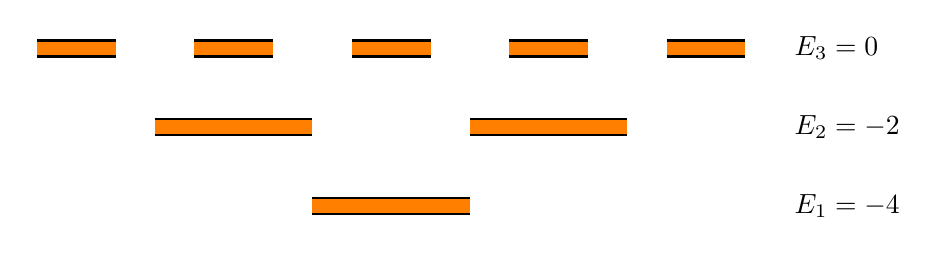
\begin{tikzpicture}
    \tikzset{level/.style   = {thick,
        double          = orange,
        double distance = 5pt,
        scale = 1.
        }}
    
    \def\Espace{9};
    \def\Gspace{11};
    
    % Draw the energy levels.
    \draw[level] (3,0)  -- (5,0) node[right]{};
    \draw[] (\Espace,0) node[right] {$E_1=-4$};
   
    \draw[level] (1,1) -- (3,1) node[right] {};
    \draw[level] (5,1) -- (7,1) node[right] {};
    \draw[] (\Espace,1) node[right] {$E_2=-2$};
    
    \def\v{.5}; 
    \draw[level] (-1+\v,2) -- (0+\v,2) node[right] {};
    \draw[level] (1+\v,2) -- (2+\v,2) node[right] {};
    \draw[level] (3+\v,2) -- (4+\v,2) node[right] {};
    \draw[level] (5+\v,2) -- (6+\v,2) node[right] {};
    \draw[level] (7+\v,2) -- (8+\v,2) node[right] {};
    \draw[] (\Espace,2) node[right] {$E_3=0$};
  \end{tikzpicture}
}


\newcommand{\TIKZgraphABC}{
  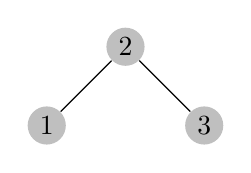
\begin{tikzpicture}[shorten >=1pt,->]
    \tikzstyle{vertex}=[circle,fill=black!25,minimum size=12pt,inner sep=2pt]
    \node[vertex] (G_1) at (-1,-1) {1};
    \node[vertex] (G_2) at (0,0)   {2};
    \node[vertex] (G_3) at (1,-1)  {3};
    \draw (G_1) -- (G_2) -- (G_3) -- cycle;
  \end{tikzpicture}
}

\newcommand{\TIKZgraphAB}{
  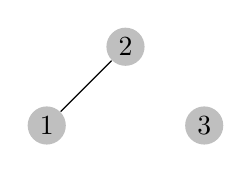
\begin{tikzpicture}[shorten >=1pt,->]
    \tikzstyle{vertex}=[circle,fill=black!25,minimum size=12pt,inner sep=2pt]
    \node[vertex] (G_1) at (-1,-1) {1};
    \node[vertex] (G_2) at (0,0)   {2};
    \node[vertex] (G_3) at (1,-1)  {3};
    \draw (G_1) -- (G_2) -- cycle;
  \end{tikzpicture}
}

\newcommand{\TIKZgraphBC}{
  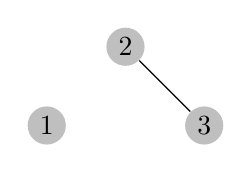
\begin{tikzpicture}[shorten >=1pt,->]
    \tikzstyle{vertex}=[circle,fill=black!25,minimum size=12pt,inner sep=2pt]
    \node[vertex] (G_1) at (-1,-1) {1};
    \node[vertex] (G_2) at (0,0)   {2};
    \node[vertex] (G_3) at (1,-1)  {3};
    \draw (G_2) -- (G_3) -- cycle;
  \end{tikzpicture}
}

\newcommand{\TIKZgraphC}{
  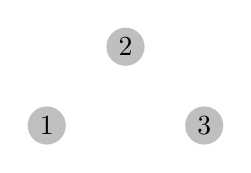
\begin{tikzpicture}[shorten >=1pt,->]
    \tikzstyle{vertex}=[circle,fill=black!25,minimum size=12pt,inner sep=2pt]
    \node[vertex] (G_1) at (-1,-1) {1};
    \node[vertex] (G_2) at (0,0)   {2};
    \node[vertex] (G_3) at (1,-1)  {3};
  \end{tikzpicture}
}


\newcommand{\TIKZgraphoneline}{
  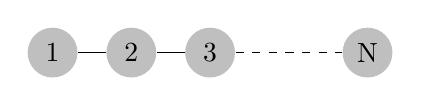
\begin{tikzpicture}[shorten >=1pt,->]
    \tikzstyle{vertex}=[circle,fill=black!25,minimum size=18pt,inner sep=2pt]
    \node[vertex] (G1) at (0,0)   {1};
    \node[vertex] (G2) at (1,0)   {2};
    \node[vertex] (G3) at (2,0)   {3};
    \node[vertex] (GN) at (4,0)   {N};
    \draw (G1) -- (G2) -- (G3) -- cycle;
    \draw[dashed] (G3) -- (GN) -- cycle;
  \end{tikzpicture}
}


\newcommand{\TIKZgraphtwoline}{
  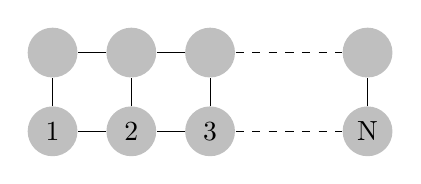
\begin{tikzpicture}[shorten >=1pt,->]
    \tikzstyle{vertex}=[circle,fill=black!25,minimum size=18pt,inner sep=2pt]
    \node[vertex] (G1) at (0,0)   {1};
    \node[vertex] (G2) at (1,0)   {2};
    \node[vertex] (G3) at (2,0)   {3};
    \node[vertex] (GN) at (4,0)   {N};
    \draw (G1) -- (G2) -- (G3) -- cycle;
    \draw[dashed] (G3) -- (GN) -- cycle;

    \node[vertex] (GN1) at (0,1)   {};
    \node[vertex] (GN2) at (1,1)   {};
    \node[vertex] (GN3) at (2,1)   {};
    \node[vertex] (G2N) at (4,1)   {};
    
    \draw (GN1) -- (GN2) -- (GN3) -- cycle;
    \draw (GN) -- (G2N) -- cycle;
    \draw (G1) -- (GN1) -- cycle;
    \draw (G2) -- (GN2) -- cycle;
    \draw (G3) -- (GN3) -- cycle;
    \draw (GN) -- (G2N) -- cycle;

    \draw[dashed] (GN3) -- (G2N) -- cycle;


  \end{tikzpicture}
}



\newcommand{\TIKZtwoladdera}{
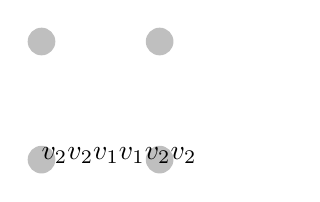
\begin{tikzpicture}[scale=\tikzpicscale]
    \node[vertex] (G1) at (0,0)   {};
    \node[vertex] (G2) at (1,0)   {};
    \node[vertex] (GA) at (0,1)   {};
    \node[vertex] (GB) at (1,1)   {};
	 \Edge[label=$v_2$](G1)(G2)
	 \Edge[label=$v_2$](GA)(GB)
	 \Edge[label=$v_1$](G1)(GA)
	 \Edge[label=$v_1$](G2)(GB)
    \node[Nvertex] (G3) at (2,0)   {};
    \node[Nvertex] (GC) at (2,1)   {};
	 \tikzstyle{EdgeStyle}=[dashed]
	 \Edge[label=$v_2$](G2)(G3)
	 \Edge[label=$v_2$](GB)(GC)
\end{tikzpicture}
}

\newcommand{\TIKZtwoladderb}{
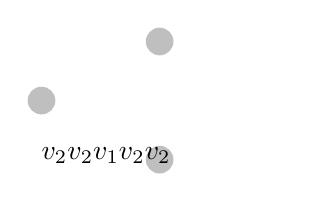
\begin{tikzpicture}[scale=\tikzpicscale]
    \node[vertex] (G2) at (1,0)   {};
    \node[vertex] (GB) at (1,1)   {};
    \node[vertex] (G1A) at (0,.5)   {};
	 \Edge[label=$v_2$](G1A)(G2)
	 \Edge[label=$v_2$](G1A)(GB)
	 \Edge[label=$v_1$](G2)(GB)
    \node[Nvertex] (G3) at (2,0)   {};
    \node[Nvertex] (GC) at (2,1)   {};
	 \tikzstyle{EdgeStyle}=[dashed]
	 \Edge[label=$v_2$](G2)(G3)
	 \Edge[label=$v_2$](GB)(GC)
\end{tikzpicture}
}

\newcommand{\TIKZtwoladderc}{
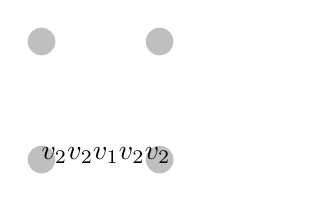
\begin{tikzpicture}[scale=\tikzpicscale]
    \node[vertex] (G1) at (0,0)   {};
    \node[vertex] (G2) at (1,0)   {};
    \node[vertex] (GA) at (0,1)   {};
    \node[vertex] (GB) at (1,1)   {};
	 \Edge[label=$v_2$](G1)(G2)
	 \Edge[label=$v_2$](GA)(GB)
	 %\Edge[label=$v_1$](G1)(GA)
	 \Edge[label=$v_1$](G2)(GB)
    \node[Nvertex] (G3) at (2,0)   {};
    \node[Nvertex] (GC) at (2,1)   {};
	 \tikzstyle{EdgeStyle}=[dashed]
	 \Edge[label=$v_2$](G2)(G3)
	 \Edge[label=$v_2$](GB)(GC)
\end{tikzpicture}
}

\newcommand{\TIKZtwoladderd}{
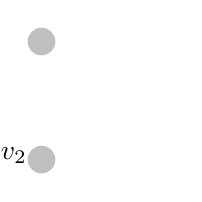
\begin{tikzpicture}[scale=\tikzpicscale]
    \node[vertex] (G2) at (1,0)   {};
    \node[vertex] (GB) at (1,1)   {};
	 %\Edge[label=$v_1$](G1)(GA)
	\tikzstyle{EdgeStyle}=[bend left]
	\Edge[label=$v_2$](G2)(GB)
  	\tikzstyle{EdgeStyle}=[bend right]
	\Edge[label=$v_1$](G2)(GB)
    \node[Nvertex] (G3) at (2,0)   {};
    \node[Nvertex] (GC) at (2,1)   {};
	 \tikzstyle{EdgeStyle}=[dashed]
	 \Edge[label=$v_2$](G2)(G3)
	 \Edge[label=$v_2$](GB)(GC)
\end{tikzpicture}
}

\newcommand{\TIKZtwoladdere}{
\begin{tikzpicture}[scale=\tikzpicscale]
    \node[vertex] (G2B) at (1,.5)   {};
	 %\Edge[label=$v_1$](G1)(GA)
	\tikzstyle{EdgeStyle}=[loop above]
	\Edge[label=$v_1$](G2B)(G2B)
   \node[Nvertex] (G3) at (2,0)   {};
   \node[Nvertex] (GC) at (2,1)   {};
	\tikzstyle{EdgeStyle}=[dashed]
	\Edge[label=$v_2$](G2B)(G3)
	\Edge[label=$v_2$](G2B)(GC)
\end{tikzpicture}
}

\newcommand{\TIKZtwoladderf}{
\begin{tikzpicture}[scale=\tikzpicscale]
    \node[vertex] (G2B) at (1,.5)   {};
   \node[Nvertex] (G3) at (2,0)   {};
   \node[Nvertex] (GC) at (2,1)   {};
	\tikzstyle{EdgeStyle}=[dashed]
	\Edge[label=$v_2$](G2B)(G3)
	\Edge[label=$v_2$](G2B)(GC)
\end{tikzpicture}
}

\newcommand{\TIKZthreeladderA}{
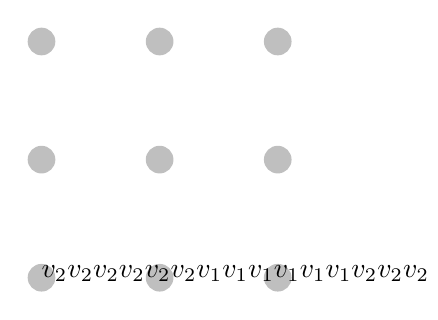
\begin{tikzpicture}[scale=\tikzpicscale]
    \node[vertex] (00) at (0,0)   {};
    \node[vertex] (10) at (1,0)   {};
	 \node[vertex] (20) at (2,0)   {};
    \node[vertex] (01) at (0,1)   {};
    \node[vertex] (11) at (1,1)   {};
    \node[vertex] (21) at (2,1)   {};
    \node[vertex] (02) at (0,2)   {};
    \node[vertex] (12) at (1,2)   {};
    \node[vertex] (22) at (2,2)   {};
	 \Edge[label=$v_2$](00)(10)
	 \Edge[label=$v_2$](10)(20)
	 \Edge[label=$v_2$](01)(11)
	 \Edge[label=$v_2$](11)(21)
	 \Edge[label=$v_2$](02)(12)
	 \Edge[label=$v_2$](12)(22)	
	 \Edge[label=$v_1$](00)(01)
	 \Edge[label=$v_1$](10)(11)
	 \Edge[label=$v_1$](20)(21)
 	 \Edge[label=$v_1$](21)(22)
 	 \Edge[label=$v_1$](11)(12)
 	 \Edge[label=$v_1$](01)(02)
    \node[Nvertex] (n30) at (3,0)   {};
    \node[Nvertex] (n31) at (3,1)   {};
    \node[Nvertex] (n32) at (3,2)   {};
	 \tikzstyle{EdgeStyle}=[dashed]
	 \Edge[label=$v_2$](20)(n30)
	 \Edge[label=$v_2$](21)(n31)
 	 \Edge[label=$v_2$](22)(n32)
\end{tikzpicture}
}

\newcommand{\TIKZthreeladderB}{
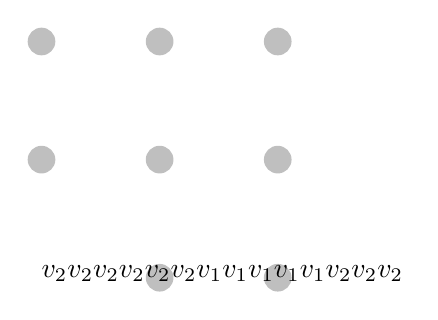
\begin{tikzpicture}[scale=\tikzpicscale]
%    \node[vertex] (00) at (0,0)   {};
    \node[vertex] (10) at (1,0)   {};
	 \node[vertex] (20) at (2,0)   {};
    \node[vertex] (01) at (0,1)   {};
    \node[vertex] (11) at (1,1)   {};
    \node[vertex] (21) at (2,1)   {};
    \node[vertex] (02) at (0,2)   {};
    \node[vertex] (12) at (1,2)   {};
    \node[vertex] (22) at (2,2)   {};
	 \Edge[label=$v_2$](01)(10)
	 \Edge[label=$v_2$](10)(20)
	 \Edge[label=$v_2$](01)(11)
	 \Edge[label=$v_2$](11)(21)
	 \Edge[label=$v_2$](02)(12)
	 \Edge[label=$v_2$](12)(22)	
%)	 \Edge[label=$v_1$](00)(01)
	 \Edge[label=$v_1$](10)(11)
	 \Edge[label=$v_1$](20)(21)
 	 \Edge[label=$v_1$](21)(22)
 	 \Edge[label=$v_1$](11)(12)
 	 \Edge[label=$v_1$](01)(02)
    \node[Nvertex] (n30) at (3,0)   {};
    \node[Nvertex] (n31) at (3,1)   {};
    \node[Nvertex] (n32) at (3,2)   {};
	 \tikzstyle{EdgeStyle}=[dashed]
	 \Edge[label=$v_2$](20)(n30)
	 \Edge[label=$v_2$](21)(n31)
 	 \Edge[label=$v_2$](22)(n32)
\end{tikzpicture}
}

\newcommand{\TIKZthreeladderC}{
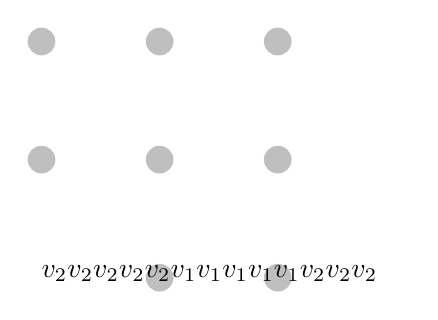
\begin{tikzpicture}[scale=\tikzpicscale]
%    \node[vertex] (00) at (0,0)   {};
    \node[vertex] (10) at (1,0)   {};
	 \node[vertex] (20) at (2,0)   {};
    \node[vertex] (01) at (0,1)   {};
    \node[vertex] (11) at (1,1)   {};
    \node[vertex] (21) at (2,1)   {};
    \node[vertex] (02) at (0,2)   {};
    \node[vertex] (12) at (1,2)   {};
    \node[vertex] (22) at (2,2)   {};
%	 \Edge[label=$v_2$](01)(10)
	 \Edge[label=$v_2$](10)(20)
	 \Edge[label=$v_2$](01)(11)
	 \Edge[label=$v_2$](11)(21)
	 \Edge[label=$v_2$](02)(12)
	 \Edge[label=$v_2$](12)(22)	
%)	 \Edge[label=$v_1$](00)(01)
	 \Edge[label=$v_1$](10)(11)
	 \Edge[label=$v_1$](20)(21)
 	 \Edge[label=$v_1$](21)(22)
 	 \Edge[label=$v_1$](11)(12)
 	 \Edge[label=$v_1$](01)(02)
    \node[Nvertex] (n30) at (3,0)   {};
    \node[Nvertex] (n31) at (3,1)   {};
    \node[Nvertex] (n32) at (3,2)   {};
	 \tikzstyle{EdgeStyle}=[dashed]
	 \Edge[label=$v_2$](20)(n30)
	 \Edge[label=$v_2$](21)(n31)
 	 \Edge[label=$v_2$](22)(n32)
\end{tikzpicture}
}

\newcommand{\TIKZthreeladderD}{
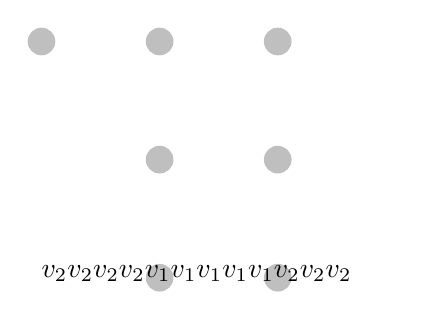
\begin{tikzpicture}[scale=\tikzpicscale]
%    \node[vertex] (00) at (0,0)   {};
    \node[vertex] (10) at (1,0)   {};
	 \node[vertex] (20) at (2,0)   {};
%    \node[vertex] (01) at (0,1)   {};
    \node[vertex] (11) at (1,1)   {};
    \node[vertex] (21) at (2,1)   {};
    \node[vertex] (02) at (0,2)   {};
    \node[vertex] (12) at (1,2)   {};
    \node[vertex] (22) at (2,2)   {};
%	 \Edge[label=$v_2$](01)(10)
	 \Edge[label=$v_2$](10)(20)
%	 \Edge[label=$v_2$](01)(11)
	 \Edge[label=$v_2$](11)(21)
	 \Edge[label=$v_2$](02)(12)
	 \Edge[label=$v_2$](12)(22)	
%)	 \Edge[label=$v_1$](00)(01)
	 \Edge[label=$v_1$](10)(11)
	 \Edge[label=$v_1$](20)(21)
 	 \Edge[label=$v_1$](21)(22)
 	 \Edge[label=$v_1$](11)(12)
 	 \Edge[label=$v_1$](11)(02)
    \node[Nvertex] (n30) at (3,0)   {};
    \node[Nvertex] (n31) at (3,1)   {};
    \node[Nvertex] (n32) at (3,2)   {};
	 \tikzstyle{EdgeStyle}=[dashed]
	 \Edge[label=$v_2$](20)(n30)
	 \Edge[label=$v_2$](21)(n31)
 	 \Edge[label=$v_2$](22)(n32)
\end{tikzpicture}
}

\newcommand{\TIKZthreeladderE}{
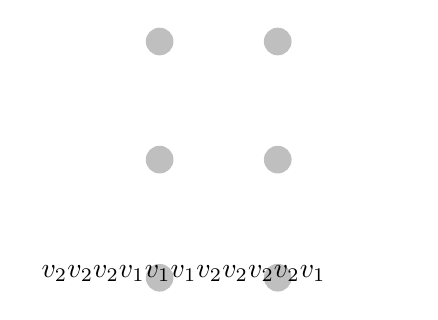
\begin{tikzpicture}[scale=\tikzpicscale]
    \node[Nvertex] (00) at (0,0)   {};
    \node[vertex] (10) at (1,0)   {};
	 \node[vertex] (20) at (2,0)   {};
%    \node[vertex] (01) at (0,1)   {};
    \node[vertex] (11) at (1,1)   {};
    \node[vertex] (21) at (2,1)   {};
%    \node[vertex] (02) at (0,2)   {};
    \node[vertex] (12) at (1,2)   {};
    \node[vertex] (22) at (2,2)   {};
%	 \Edge[label=$v_2$](01)(10)
	 \Edge[label=$v_2$](10)(20)
%	 \Edge[label=$v_2$](01)(11)
	 \Edge[label=$v_2$](11)(21)
%	 \Edge[label=$v_2$](02)(12)
	 \Edge[label=$v_2$](12)(22)	
%)	 \Edge[label=$v_1$](00)(01)
	 \Edge[label=$v_1$](10)(11)
	 \Edge[label=$v_1$](20)(21)
 	 \Edge[label=$v_1$](21)(22)
% 	 \Edge[label=$v_1$](11)(02)
    \node[Nvertex] (n30) at (3,0)   {};
    \node[Nvertex] (n31) at (3,1)   {};
    \node[Nvertex] (n32) at (3,2)   {};
	 \tikzstyle{EdgeStyle}=[dashed]
	 \Edge[label=$v_2$](20)(n30)
	 \Edge[label=$v_2$](21)(n31)
 	 \Edge[label=$v_2$](22)(n32)
 	 \tikzstyle{EdgeStyle}=[bend left]
  	 \Edge[label=$v_2$](11)(12)
  	 \tikzstyle{EdgeStyle}=[bend right]
  	 \Edge[label=$v_1$](11)(12)
\end{tikzpicture}
}

\newcommand{\TIKZthreeladderF}{
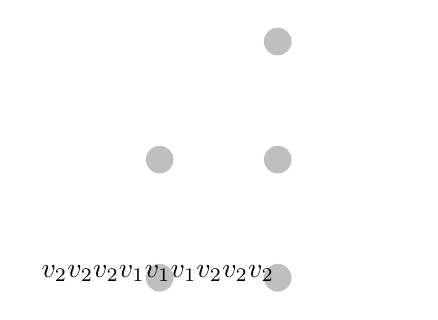
\begin{tikzpicture}[scale=\tikzpicscale]
    \node[Nvertex] (00) at (0,0)   {};
    \node[vertex] (10) at (1,0)   {};
	 \node[vertex] (20) at (2,0)   {};
%    \node[vertex] (01) at (0,1)   {};
    \node[vertex] (11) at (1,1)   {};
    \node[vertex] (21) at (2,1)   {};
%    \node[vertex] (02) at (0,2)   {};
%    \node[vertex] (12) at (1,2)   {};
    \node[vertex] (22) at (2,2)   {};
%	 \Edge[label=$v_2$](01)(10)
	 \Edge[label=$v_2$](10)(20)
%	 \Edge[label=$v_2$](01)(11)
	 \Edge[label=$v_2$](11)(21)
%	 \Edge[label=$v_2$](02)(12)
	 \Edge[label=$v_2$](11)(22)	
%)	 \Edge[label=$v_1$](00)(01)
	 \Edge[label=$v_1$](10)(11)
	 \Edge[label=$v_1$](20)(21)
 	 \Edge[label=$v_1$](21)(22)
% 	 \Edge[label=$v_1$](11)(02)
    \node[Nvertex] (n30) at (3,0)   {};
    \node[Nvertex] (n31) at (3,1)   {};
    \node[Nvertex] (n32) at (3,2)   {};
	 \tikzstyle{EdgeStyle}=[dashed]
	 \Edge[label=$v_2$](20)(n30)
	 \Edge[label=$v_2$](21)(n31)
 	 \Edge[label=$v_2$](22)(n32)
  	 %\tikzstyle{EdgeStyle}=[loop above]
  	 %\Edge[label=$v_1$](11)(11)
\end{tikzpicture}
}

\newcommand{\TIKZthreeladderG}{
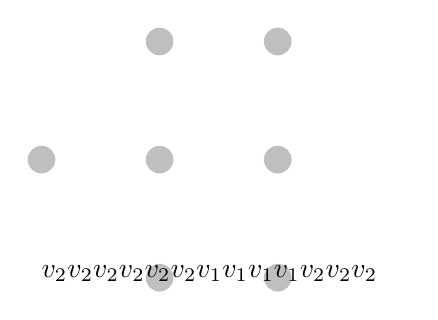
\begin{tikzpicture}[scale=\tikzpicscale]
%    \node[vertex] (00) at (0,0)   {};
    \node[vertex] (10) at (1,0)   {};
	 \node[vertex] (20) at (2,0)   {};
    \node[vertex] (01) at (0,1)   {};
    \node[vertex] (11) at (1,1)   {};
    \node[vertex] (21) at (2,1)   {};
%    \node[vertex] (02) at (0,2)   {};
    \node[vertex] (12) at (1,2)   {};
    \node[vertex] (22) at (2,2)   {};
	 \Edge[label=$v_2$](01)(10)
	 \Edge[label=$v_2$](10)(20)
	 \Edge[label=$v_2$](01)(11)
	 \Edge[label=$v_2$](11)(21)
	 \Edge[label=$v_2$](01)(12)
	 \Edge[label=$v_2$](12)(22)	
%)	 \Edge[label=$v_1$](00)(01)
	 \Edge[label=$v_1$](10)(11)
	 \Edge[label=$v_1$](20)(21)
 	 \Edge[label=$v_1$](21)(22)
 	 \Edge[label=$v_1$](11)(12)
% 	 \Edge[label=$v_1$](01)(02)
    \node[Nvertex] (n30) at (3,0)   {};
    \node[Nvertex] (n31) at (3,1)   {};
    \node[Nvertex] (n32) at (3,2)   {};
	 \tikzstyle{EdgeStyle}=[dashed]
	 \Edge[label=$v_2$](20)(n30)
	 \Edge[label=$v_2$](21)(n31)
 	 \Edge[label=$v_2$](22)(n32)
\end{tikzpicture}
}

\newcommand{\TIKZthreeladderH}{
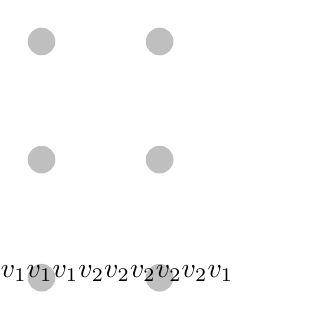
\begin{tikzpicture}[scale=\tikzpicscale]
%    \node[vertex] (00) at (0,0)   {};
    \node[vertex] (10) at (1,0)   {};
	 \node[vertex] (20) at (2,0)   {};
%    \node[vertex] (01) at (0,1)   {};
    \node[vertex] (11) at (1,1)   {};
    \node[vertex] (21) at (2,1)   {};
%    \node[vertex] (02) at (0,2)   {};
    \node[vertex] (12) at (1,2)   {};
    \node[vertex] (22) at (2,2)   {};
	 \Edge[label=$v_2$](10)(20)
%	 \Edge[label=$v_2$](01)(11)
	 \Edge[label=$v_2$](11)(21)
%	 \Edge[label=$v_2$](01)(12)
	 \Edge[label=$v_2$](12)(22)	
%)	 \Edge[label=$v_1$](00)(01)
	 \Edge[label=$v_1$](20)(21)
 	 \Edge[label=$v_1$](21)(22)
 	 \Edge[label=$v_1$](11)(12)
% 	 \Edge[label=$v_1$](01)(02)
    \node[Nvertex] (n30) at (3,0)   {};
    \node[Nvertex] (n31) at (3,1)   {};
    \node[Nvertex] (n32) at (3,2)   {};
	 \tikzstyle{EdgeStyle}=[dashed]
	 \Edge[label=$v_2$](20)(n30)
	 \Edge[label=$v_2$](21)(n31)
 	 \Edge[label=$v_2$](22)(n32)
 	 
 	 \tikzstyle{EdgeStyle}=[bend left]
 	 \Edge[label=$v_2$](10)(11)
  	 \tikzstyle{EdgeStyle}=[bend left=50]
 	 \Edge[label=$v_2$](10)(12)
  	 %\Edge[label=$v_2$](11)(12)
 	 \tikzstyle{EdgeStyle}=[bend right]
	 \Edge[label=$v_1$](10)(11)
\end{tikzpicture}
}

\newcommand{\TIKZthreeladderI}{
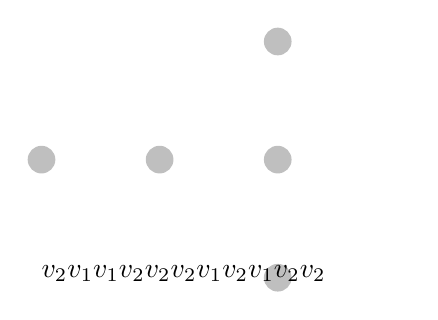
\begin{tikzpicture}[scale=\tikzpicscale]
%    \node[vertex] (00) at (0,0)   {};
%    \node[vertex] (10) at (1,0)   {};
	 \node[vertex] (20) at (2,0)   {};
    \node[vertex] (01) at (0,1)   {};
    \node[vertex] (11) at (1,1)   {};
    \node[vertex] (21) at (2,1)   {};
%    \node[vertex] (02) at (0,2)   {};
%    \node[vertex] (12) at (1,2)   {};
    \node[vertex] (22) at (2,2)   {};
%	 \Edge[label=$v_2$](01)(10)
%	 \Edge[label=$v_2$](10)(20)
%	 \Edge[label=$v_2$](01)(21)
	 \Edge[label=$v_2$](11)(21)
%	 \Edge[label=$v_2$](12)(22)	
%)	 \Edge[label=$v_1$](00)(01)
%	 \Edge[label=$v_1$](10)(11)
	 \Edge[label=$v_1$](20)(21)
 	 \Edge[label=$v_1$](21)(22)
% 	 \Edge[label=$v_1$](11)(12)
% 	 \Edge[label=$v_1$](01)(02)
    \node[Nvertex] (n30) at (3,0)   {};
    \node[Nvertex] (n31) at (3,1)   {};
    \node[Nvertex] (n32) at (3,2)   {};
	 \tikzstyle{EdgeStyle}=[dashed]
	 \Edge[label=$v_2$](20)(n30)
	 \Edge[label=$v_2$](21)(n31)
 	 \Edge[label=$v_2$](22)(n32)

	 \tikzstyle{EdgeStyle}=[]
	 \Edge[label=$v_1$](01)(11)
  	 \tikzstyle{EdgeStyle}=[bend left=50]
	 \Edge[label=$v_2$](01)(22)
 	 \Edge[label=$v_1$](01)(11)
  	 \tikzstyle{EdgeStyle}=[bend right=50]
 	 \Edge[label=$v_2$](01)(20)
 	 \Edge[label=$v_2$](01)(11)
\end{tikzpicture}
}


\newcommand{\TIKZthreeladderJ}{
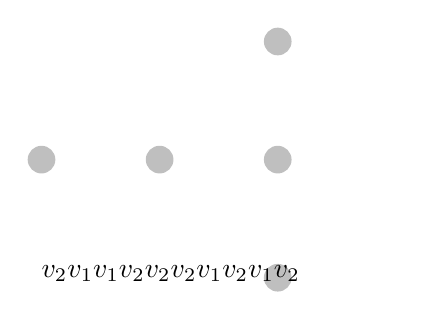
\begin{tikzpicture}[scale=\tikzpicscale]
%    \node[vertex] (00) at (0,0)   {};
%    \node[vertex] (10) at (1,0)   {};
	 \node[vertex] (20) at (2,0)   {};
    \node[vertex] (01) at (0,1)   {};
    \node[vertex] (11) at (1,1)   {};
    \node[vertex] (21) at (2,1)   {};
%    \node[vertex] (02) at (0,2)   {};
%    \node[vertex] (12) at (1,2)   {};
    \node[vertex] (22) at (2,2)   {};
%	 \Edge[label=$v_2$](01)(10)
%	 \Edge[label=$v_2$](10)(20)
%	 \Edge[label=$v_2$](01)(21)
	 \Edge[label=$v_2$](11)(21)
%	 \Edge[label=$v_2$](12)(22)	
%)	 \Edge[label=$v_1$](00)(01)
%	 \Edge[label=$v_1$](10)(11)
	 \Edge[label=$v_1$](20)(21)
 	 \Edge[label=$v_1$](21)(22)
% 	 \Edge[label=$v_1$](11)(12)
% 	 \Edge[label=$v_1$](01)(02)
    \node[Nvertex] (n30) at (3,0)   {};
    \node[Nvertex] (n31) at (3,1)   {};
    \node[Nvertex] (n32) at (3,2)   {};
	 \tikzstyle{EdgeStyle}=[dashed]
	 \Edge[label=$v_2$](20)(n30)
	 \Edge[label=$v_2$](21)(n31)
 	 \Edge[label=$v_2$](22)(n32)

	 \tikzstyle{EdgeStyle}=[]
	 \Edge[label=$v_1$](01)(11)
  	 \tikzstyle{EdgeStyle}=[bend left=50]
	 \Edge[label=$v_2$](01)(22)
 	 \Edge[label=$v_1$](01)(11)
  	 \tikzstyle{EdgeStyle}=[bend right=50]
 	 \Edge[label=$v_2$](01)(20)
% 	 \Edge[label=$v_2$](01)(11)
\end{tikzpicture}
}

\newcommand{\TIKZoneladderA}{
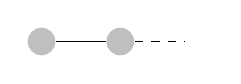
\begin{tikzpicture}[shorten >=1pt,->]
    \tikzstyle{vertex}=[circle,fill=black!25,minimum size=10pt,inner sep=2pt]
    \tikzstyle{nullvertex}=[circle,fill=white!25,minimum size=10pt,inner sep=2pt]
    \node[vertex] (G1) at (0,0)   {};
    \node[vertex] (G2) at (1,0)   {};
    \node[nullvertex] (GX) at (2,0)   {};
    \draw (G1) -- (G2) -- cycle;
    \draw[dashed] (G2) -- (GX) -- cycle;
\end{tikzpicture}
}

\newcommand{\TIKZoneladderB}{
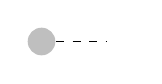
\begin{tikzpicture}[shorten >=1pt,->]
    \tikzstyle{vertex}=[circle,fill=black!25,minimum size=10pt,inner sep=2pt]
    \tikzstyle{nullvertex}=[circle,fill=white!25,minimum size=10pt,inner sep=2pt]
    \node[vertex] (G2) at (1,0)   {};
    \node[nullvertex] (GX) at (2,0)   {};
    \draw[dashed] (G2) -- (GX) -- cycle;
\end{tikzpicture}
}

\newcommand{\TIKZoneladderC}{

\begin{tikzpicture}[shorten >=1pt,->]
    \tikzstyle{vertex}=[circle,fill=black!25,minimum size=10pt,inner sep=2pt]
    \tikzstyle{nullvertex}=[circle,fill=white!25,minimum size=10pt,inner sep=2pt]
    \node[vertex] (G1) at (0,0)   {};
    \node[vertex] (G2) at (1,0)   {};
    \node[nullvertex] (GX) at (2,0)   {};
    %\draw (G1) -- (G2) -- cycle;
    \draw[dashed] (G2) -- (GX) -- cycle;
\end{tikzpicture}
}

\newcommand{\TIKZpetersengraph} {
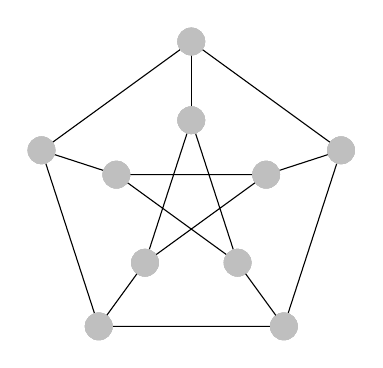
\begin{tikzpicture}[]
    \tikzstyle{vertex}=[circle,fill=black!25,minimum size=10pt,inner sep=2pt]
            
\draw (18:2cm) -- (90:2cm) -- (162:2cm) -- (234:2cm) -- (306:2cm) -- cycle;
\draw (18:1cm) -- (162:1cm) -- (306:1cm) -- (90:1cm) -- (234:1cm) -- cycle;
\foreach \x in {18,90,162,234,306}{
\draw (\x:1cm) -- (\x:2cm);

    \node[vertex] at (18:2cm) {};
    \node[vertex] at (90:2cm) {};
    \node[vertex] at (162:2cm) {};
    \node[vertex] at (234:2cm) {};
    \node[vertex] at (306:2cm) {};
    \node[vertex] at (18:1cm) {};
    \node[vertex] at (162:1cm) {};
    \node[vertex] at (306:1cm) {};
    \node[vertex] at (90:1cm) {};
    \node[vertex] at (234:1cm) {};

%\draw (\x:2cm) circle (2pt);
%\draw (\x:1cm) circle (2pt);
}
\end{tikzpicture}
}

\newcommand{\TIKZFLWmacrostates} {

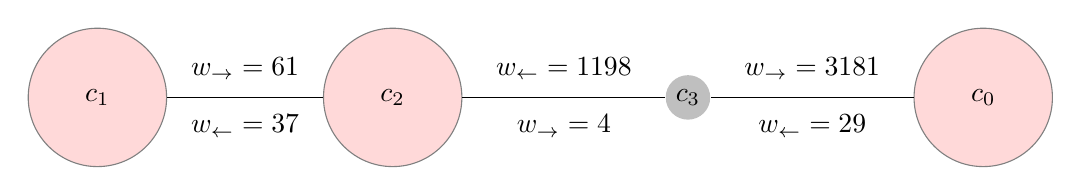
\begin{tikzpicture}[scale=\tikzpicscale]

  \node[big_vertex] (c1) at (0,0)   {$c_1$};
  \node[big_vertex] (c2) at (1*\vertexshiftamount,0)   {$c_2$};
  \node[vertex]    (c3) at (2*\vertexshiftamount,0)   {$c_3$};
  \node[big_vertex] (c0) at (3*\vertexshiftamount,0)   {$c_0$};
  
  \draw [] (c0) -> node[above=.1cm] {$w_{\rightarrow}=3181$} (c3);
  \draw [] (c0) -> node[below=.1cm] {$w_{\leftarrow}=29$} (c3);

  \draw [] (c2) -> node[above=.1cm] {$w_{\leftarrow}=1198$} (c3);  
  \draw [] (c2) -> node[below=.1cm] {$w_{\rightarrow}=4$} (c3);
  
  \draw [] (c2) -- node[below=.1cm] {$w_{\leftarrow}=37$} (c1);
  \draw [] (c2) -- node[above=.1cm] {$w_{\rightarrow}=61$} (c1);
\end{tikzpicture}
}

\newcommand{\TIKZbetahairpinNativestate} {
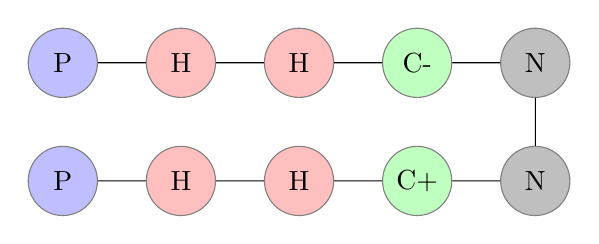
\begin{tikzpicture}[scale=\tikzpicscale]
    \tikzstyle{hvertex}=[circle,fill=red!25,minimum size=25pt,inner sep=2pt,draw=black!50]
    \tikzstyle{pvertex}=[circle,fill=blue!25,minimum size=25pt,inner sep=2pt,draw=black!50]
    \tikzstyle{cpvertex}=[circle,fill=green!25,minimum size=25pt,inner sep=2pt,draw=black!50]
    \tikzstyle{nvertex}=[circle,fill=black!25,minimum size=25pt,inner sep=2pt,draw=black!50]

    \node[pvertex] (r0) at (0,0)   {\chem{P}};
    \node[hvertex] (r1) at (1,0)   {\chem{H}};
    \node[hvertex] (r2) at (2,0)   {\chem{H}};
    \node[cpvertex] (r3) at (3,0)   {\chem{C+}};
    \node[nvertex] (r4) at (4,0)   {\chem{N}};
    \node[nvertex] (r5) at (4,1)   {\chem{N}};
    \node[cpvertex] (r6) at (3,1)   {\chem{C-}};
    \node[hvertex] (r7) at (2,1)   {\chem{H}};
    \node[hvertex] (r8) at (1,1)   {\chem{H}};
    \node[pvertex] (r9) at (0,1)   {\chem{P}};

    \draw [] (r0)--(r1)--(r2)--(r3)--(r4)--(r5)--(r6)--(r7)--(r8)--(r9)--cycle;
   
\end{tikzpicture}
}


\newcommand{\TIKZbetahairpinMacrostates} {
\begin{tikzpicture}[scale=\tikzpicscale]
    \node[macrostate_vertex] (R) at (0,0)   {
    \begin{minipage}{3.1cm}
    \includegraphics[width=1.5 cm]{supplement/beta_cluster_example_2/pictures/21/state_cluster_shapes_150.pdf} 
    \includegraphics[width=1.5 cm]{supplement/beta_cluster_example_2/pictures/21/state_cluster_shapes_17.pdf} \\
    \includegraphics[width=1.5 cm]{supplement/beta_cluster_example_2/pictures/21/state_cluster_shapes_32.pdf} 
    \includegraphics[width=1.5 cm]{supplement/beta_cluster_example_2/pictures/21/state_cluster_shapes_200.pdf} \\
  	 $c_\chem{R}$ random coil
    \end{minipage}
    };
    \node[macrostate_vertex] (I) at (1.5*\vertexshiftamount,0)   {
    \begin{minipage}{3.1cm} \centering
    \includegraphics[width=2 cm]{supplement/beta_cluster_example_2/pictures/saved_macrostates/intermed.png} \\
  	 $c_\chem{I}$ intermediate \\ (turn formation)
    \end{minipage}
	 };
    \node[macrostate_vertex] (F) at (3*\vertexshiftamount,0)   
    {
    \begin{minipage}{3.1cm} \centering
    \includegraphics[width=2.5 cm]{supplement/beta_cluster_example_2/pictures/saved_macrostates/native.png} \\
  	 $c_\chem{F}$ native state
    \end{minipage}
    };

  \tikzstyle{EdgeStyle}=[bend right]
  \Edge[label=$\B{S}_{\chem{R I}}$](R)(I)
  \Edge[label=$\B{S}_{\chem{I R}}$](I)(R)
  
  \tikzstyle{EdgeStyle}=[]
  \Edge[label=$\B{S}_{\chem{I F}}$](I)(F)
  
\end{tikzpicture}
}


%\end{comment}


% Convenience functions
\newcommand{\B}[1]{ {\bf #1} }      		% Bold text for matrices
\newcommand{\Z}{\mathcal{Z}}				% Partition function
\newcommand{\HAM}{\mathcal{H}}		% Hamiltonian
\newcommand{\qp}[0]{(\B{q},\B{p})}  % Cannonical variables (q,p) 
\newcommand{\pfrac}[2]{\frac{\partial #1}{\partial #2}} 	% partial 1 /partial 2 
\newcommand{\ket}[1]  {\left | \, #1 \right \rangle}			% bra-ket notation
\newcommand{\abs}[1]{\left\vert #1 \right\vert}		% vert bars for averages
\newcommand{\norm}[1]{\left\Vert #1 \right\Vert}	% taller vert bars for the norm
\newcommand{\evalat}[1]{\left. #1 \right \vert}	% ex. evaluating the int. at its limits
\newcommand{\set}[1]{\left\{ #1 \right\}}					% squigle brackets for sets
\newcommand{\avg}[1]{\left< #1 \right>}					% angle brackets for averages
\newcommand{\paren}[1]{\left( #1 \right)}					% grows parentheses to the correct size
\newcommand{\brackets}[1]{\left[ #1 \right]}			% grows square brackets
\newcommand{\braces}[1]{\left \{ #1 \right \}}
\newcommand{\piecewisebrace}[1]{\left \{ #1 \right .} % Useful for piecewise functions



% Macro for table stre
\newcommand{\ra}[1]{\renewcommand{\arraystretch}{#1}}
\newcommand{\Go}{\text{G}\bar{\text{o}}}
\newcommand{\GO}{\textbf{G}}
\newcommand{\CHI}{\mathbf{X}}
\newcommand{\KP}{k_+}
\newcommand{\KM}{k_-}
\newcommand{\KPMAX}{k_+^*}

\newcommand{\paperrefA}{Hoppe and Yuan, J. Phys. Chem. B, 115(9), pg $2006-2013$ (2011)}
\newcommand{\paperrefB}{Hoppe and Yuan, Phys. Rev. E 80, 011404 (2009)}

%\logo{
\includegraphics[height=1.6cm]{Drexel_University.pdf}}

\title[Protein Folding with Implicit Crowders]
{

\includegraphics[height=.7\textheight]{block_text_creation/text_block.pdf}
}
%\author{Travis Hoppe{\\ \emph{hoppe@drexel.edu}}}
{
%Drexel University \\
%\medskip
%}
\date{}


%\usepackage{handoutWithNotes}
%\pgfpagesuselayout{2 on 1 with notes landscape}[a4paper,border shrink=5mm]


\begin{document}

\begin{frame}
	\thispagestyle{empty}
	\titlepage
\end{frame}

\frame{
	\frametitle{Outline}
	\tableofcontents
	\thispagestyle{empty}
}

\section{Introduction}

\setcounter{framenumber}{0}

\begin{frame}
	\frametitle{Protein Folding}
	\begin{block}{Proteins}
	\begin{itemize}
	\item Responsible for wide variety of biological function
	\item Linear polymer chains of amino acids
	\end{itemize}	
	\end{block}
	
	\begin{block}{Folding}
	\begin{itemize}
	\item Central problem: from primary sequence and physiological conditions determine the \emph{unique} native state
	\item Misfolding and aggregation results in many clinical disorders including neurodegenerative disorders like Huntington's and Alzheimer's disease and diabetes.
	\end{itemize}	
	\end{block}

\end{frame}

\begin{frame}
	\frametitle{Entropy: The Science of Counting}

\begin{block}{Equilibrium statistical mechanics}
\[
\scalebox{2.0}{$
Z = \sum g(E_i) e^{-\beta E_i}$} 
\] \\
\begin{itemize}
\item The partition function gives a complete description of the system.
$$S = k \ln g(E) $$
\item Try to solve for the density of states directly!
\end{itemize}
\end{block}
%
\pause
%
\textbf{Example:} \\
\begin{center}
\scalebox{.8}{\TIKZenergylevelSHORT} 
\end{center}
This gives a DOS of $g(-4)=1$, $g(-2)=2$, $g(0)=5$.

\end{frame}

\begin{comment}
\begin{frame}
	\frametitle{The perception of Biophysics}
	\begin{center}
	\begin{tabular}{ l c l }
	{\Huge BIO}physics & {\hspace{2.5em} \Huge $\Longleftrightarrow$ } & \hspace{1em} bio{\Huge PHYSICS} \\
	\end{tabular}
	\end{center}
	%\pause
	\begin{center}
	\begin{tabular}{ c c c }
	& \hspace{12em} & \\
	Function & & Matter \\
	Growth && Energy \\
	Taxonomy && Force \\
	\end{tabular}
	\end{center}

	\begin{center}
	\begin{tabular}{ c c c }
	& \hspace{4em} & \\
	Optical/Electron Microscopes & & X-Ray Crystallography \\
	Gel Electrophoresis &&  Atomic Force Microscopy \\
	\end{tabular}
	\end{center}
\end{frame}
\end{comment}

\section{Crowding Effects}

\frame{
\frametitle{What is Crowding?}
\begin{center}
\hspace{2em}
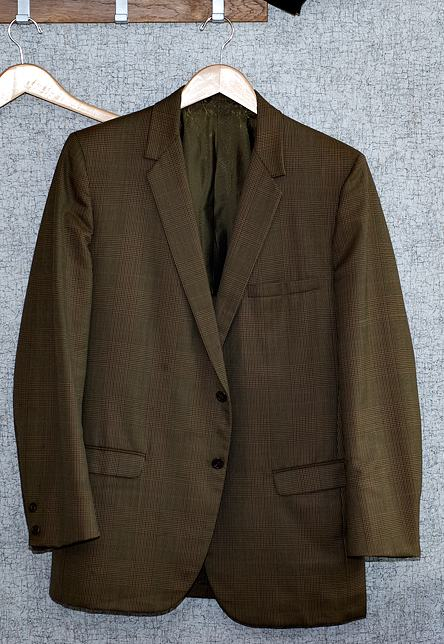
\includegraphics[height=2.8cm]{pictures/jacket.jpg}
\mbox{ \hspace{2em} \raisebox{3em}{\Huge{$\Rightarrow$}}\hspace{1em} }
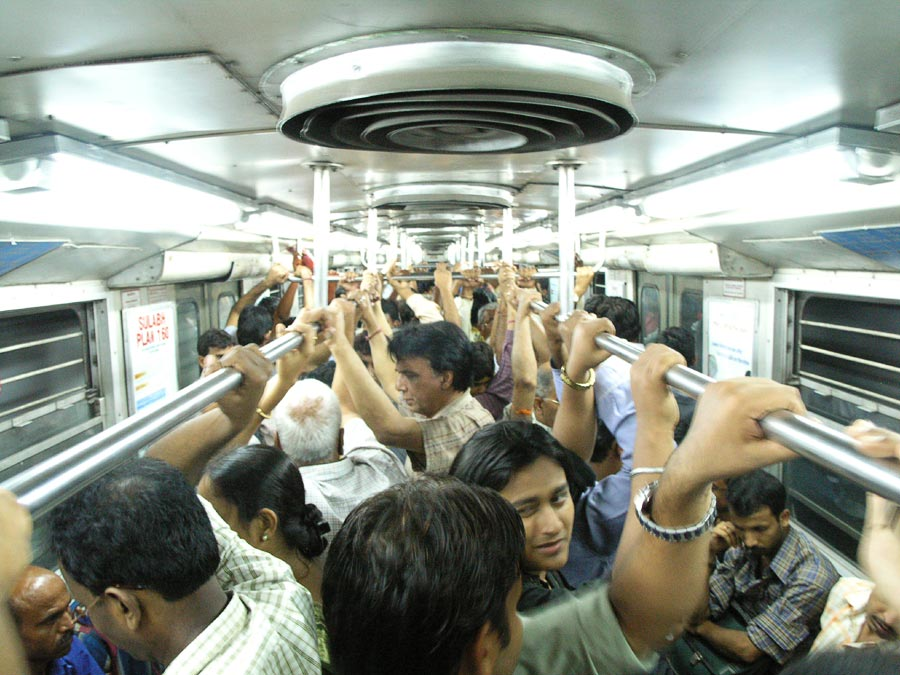
\includegraphics[height=2.8cm]{pictures/subway.jpg}
\vspace{1.5em}
\newline
%\pause
\vspace{.5em}
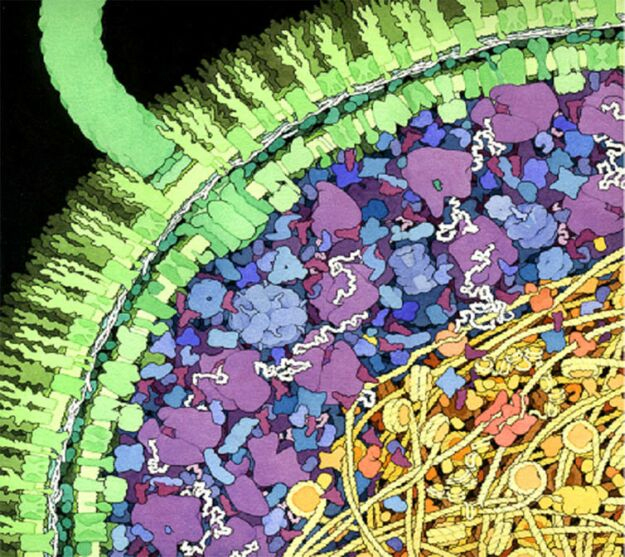
\includegraphics[height=3cm]{pictures/crowding_JMB.jpg}
\end{center}

\begin{center}
\textbf{Crowding reduces the conformational state space of the peptide.}
\end{center}
}

\frame{
\frametitle{Crowding Induced Function Change\footnote{Dhar, Gruebele, Cheung, et. al., PNAS 107, 17586 (2010)}
}

\begin{center}
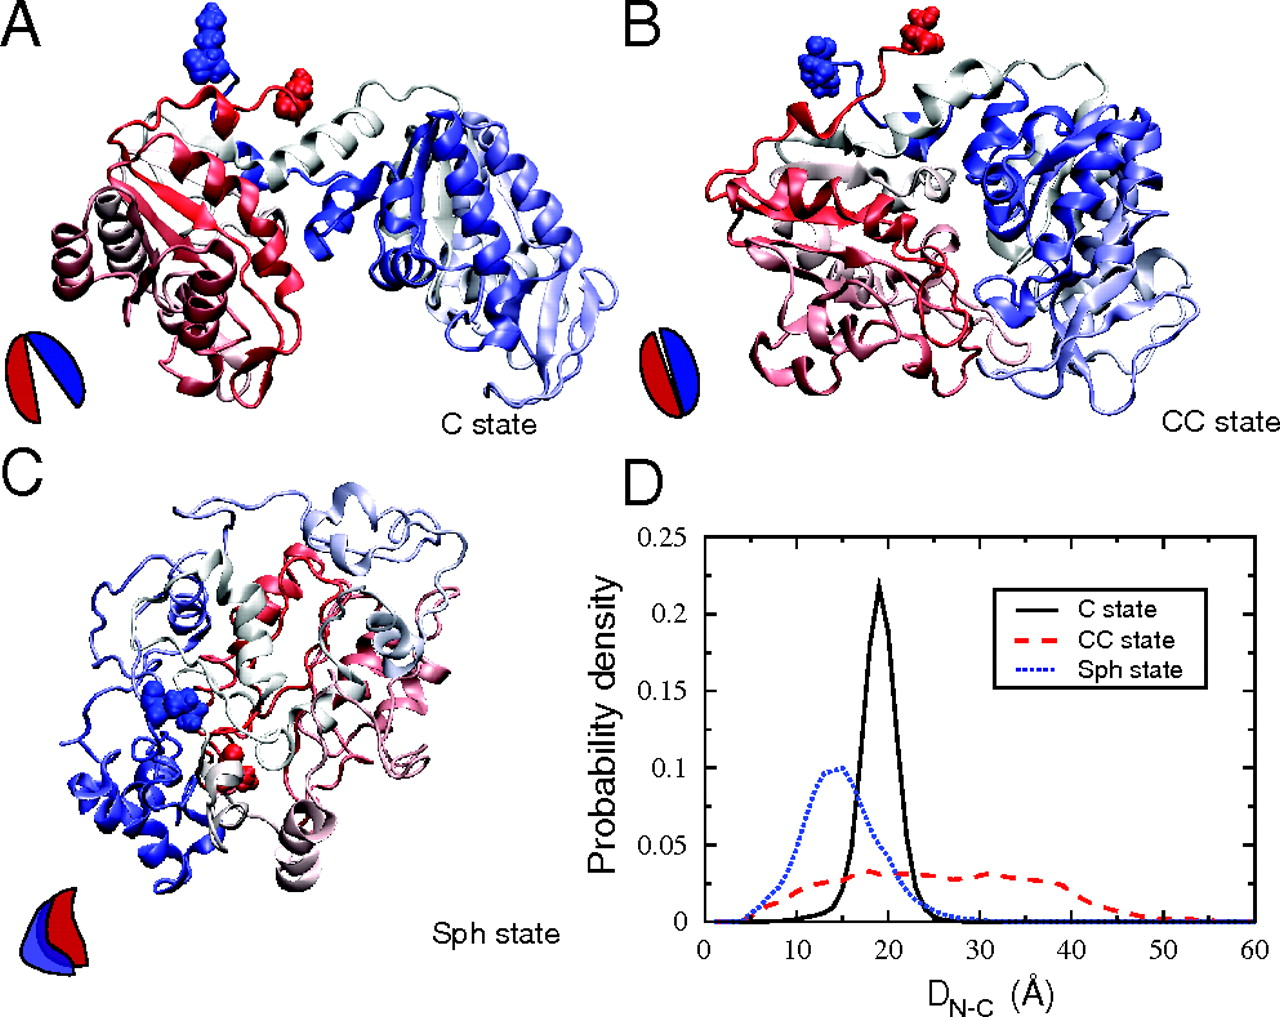
\includegraphics[height=5cm]{pictures/cheung_large.jpg}
\end{center}

\textbf{Crowding changes activity rates and function,}
\newline
\textbf{and may change the native state}

}

\frame{
\frametitle{Hard-Sphere Experiments, Crowding Insights}

\begin{centering}
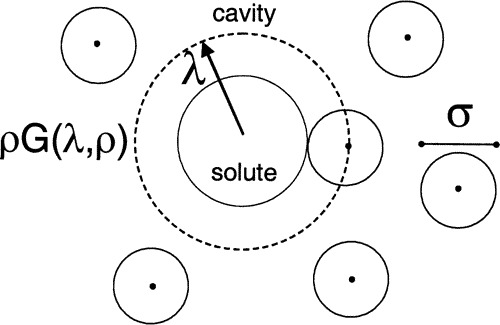
\includegraphics[width=5cm]{pictures/depzone.jpg}\\
{\footnotesize Picture from [Heying, 2004], depletion zone traced with dashed lines} \\
\end{centering}

\vspace{2em}
Hard-sphere studies of the crowding effect have shown:
\begin{itemize}
\item \textbf{Changes of the conformations of the cosolute}
\item \textbf{Motion towards minimal curvature}
\end{itemize}

}


\frame{
\frametitle{Crowding Induced Cosolute Conformation\footnote{\paperrefB}}

\begin{center}
\includegraphics[width=5.5cm]{../entropic_flow_paper/FIG1_EDIT.jpg}
\hspace{1em}
\includegraphics[width=5.5cm]{../entropic_flow_paper/FIG2_EDIT.jpg}
\end{center}

\begin{center}
Hard-sphere experiments with fixed inner elliptical boundary shows standard radial density profiles
\end{center}
}


\frame{
\frametitle{Crowding Induced Flow\footnote[5]{\paperrefB}}

\begin{center}
{\bf Non-spherical  objects generate flows from random initial conditions!}\\
\includegraphics[width=7cm]{../entropic_flow_paper/FIG3_fourvelocity.jpg} \\
Four vortices of paired spins, net angular momentum is still conserved \\ 
Effect: Crowding induced shape change 
(also considered by Cheung\footnote{Cheung and Thirumalai, J. Phys. Chem. B, 111, 8250-8257 (2007)})
\end{center}

}


\frame{
\frametitle{Scaled Particle Theory}
\begin{itemize}
\item Measures the cost of inserting a new particle into a solution
\item Rigorous results known for binary hard-sphere solutions
\item Extended to aspherical particles by Kihara\footnote{Kihara, Rev. Mod. Phys. 25, 831 (1953)} 
\item Aspherical SPT for proteins by Minton\footnote{Minton, Method Enzymol. 295, 127 (1998)}
\end{itemize}
}

\section{Experimental starting points}

\begin{frame}
\frametitle{Designed \texorpdfstring{$\beta$}{Beta}-sheet peptides}
Collection of experiments by Feng Gai at U. Penn.
\vspace{1em}
\begin{block}
{Properties:}
\begin{itemize}
\item $\beta$-sheet motif
\item Low aggregation propensity
\item Known native-state
\end{itemize}
\end{block}


\begin{block} {}
\begin{itemize}
\item \#1 RFSEV$^D$[PG]KKFITS$^D$[PG]KTYTEV$^D$[PG]KKILQ\footnotemark
\item \#2 RFIEV$^D$[PG]KKFITS$^D$[PG]KTYTE\footnotemark
\end{itemize}
\raggedleft \footnotesize{$^D$P = D-Pro}
\end{block}

\footnotetext[1]{Xu, Gai, et. al., Biochem.47, 2064 (2008)}
\footnotetext[2]{Hudson and Anderson, Biopolymers.83(4) pg. 424-433 (2006)}
\end{frame}


\begin{frame}
\frametitle{Native state representation}


\begin{block}
{Wild-type \texorpdfstring{$\beta$}{Beta}-sheet peptide (trpzip-m1)}
\begin{itemize}
\item \#3 GEWTWAD[AT]KTWTWTE\footnotemark
\end{itemize}
\end{block}
\footnotetext[3]{Du, Gai, et. al. Biochem.45, 2668(2006)}
\vspace{1em}
\begin{figure}[ht]
 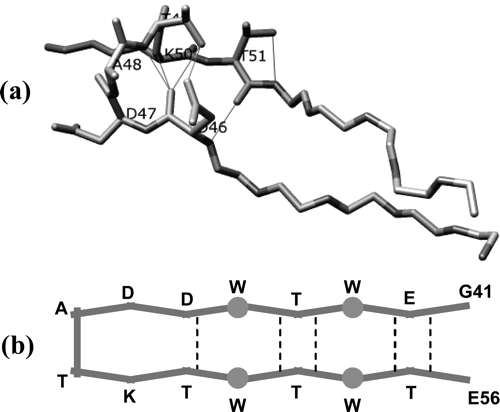
\includegraphics[width=4cm]{pictures/16_resiude_seq_chem_sch.png}\hspace{1em}
 \includegraphics[width=5cm]{../WL_crowding_paper/PIC_28_residue_seq_chem_sch.png}
\caption{\raggedright Native state of the wild-type 16-residue and designed 28-residue peptides represented schematically.}
\end{figure}

\end{frame}


\begin{frame}
\frametitle{Why study these peptides?}

\begin{itemize}
\item Thermal transition data 
\item Crowding data under equilibrium properties
\end{itemize}

\begin{center}
%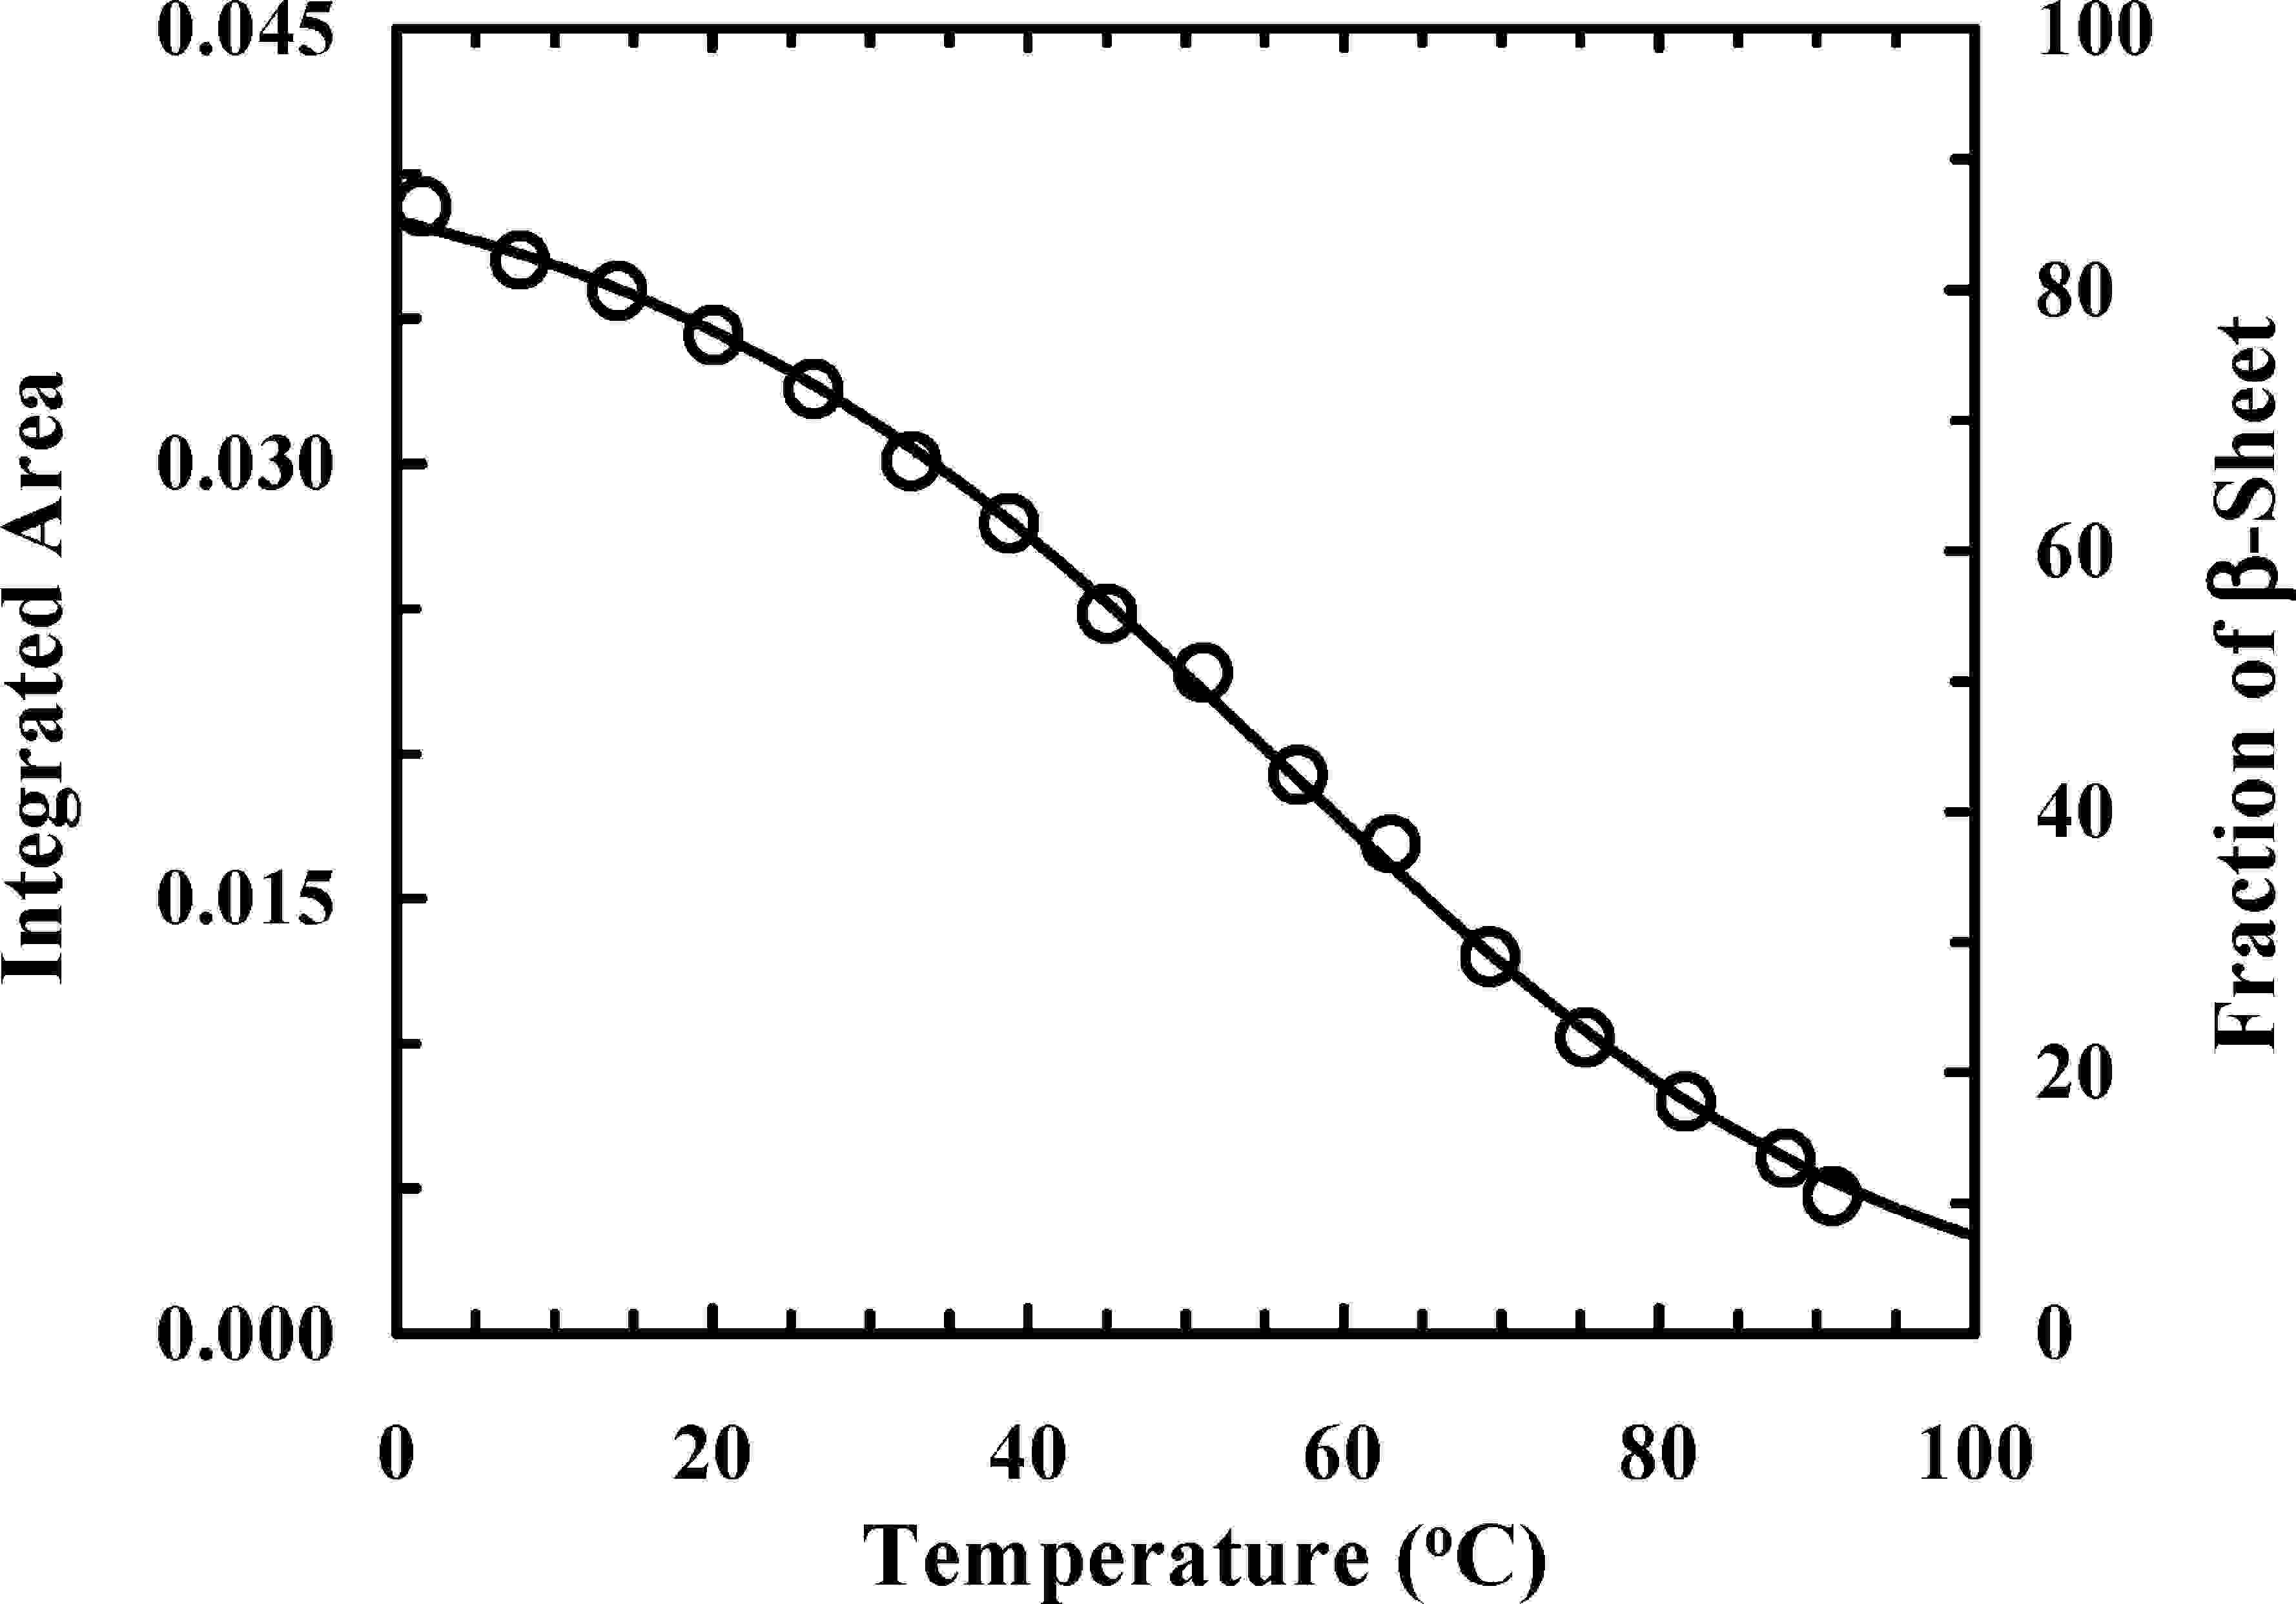
\includegraphics[width=5cm]{pictures/20aa_ff_low.jpg}
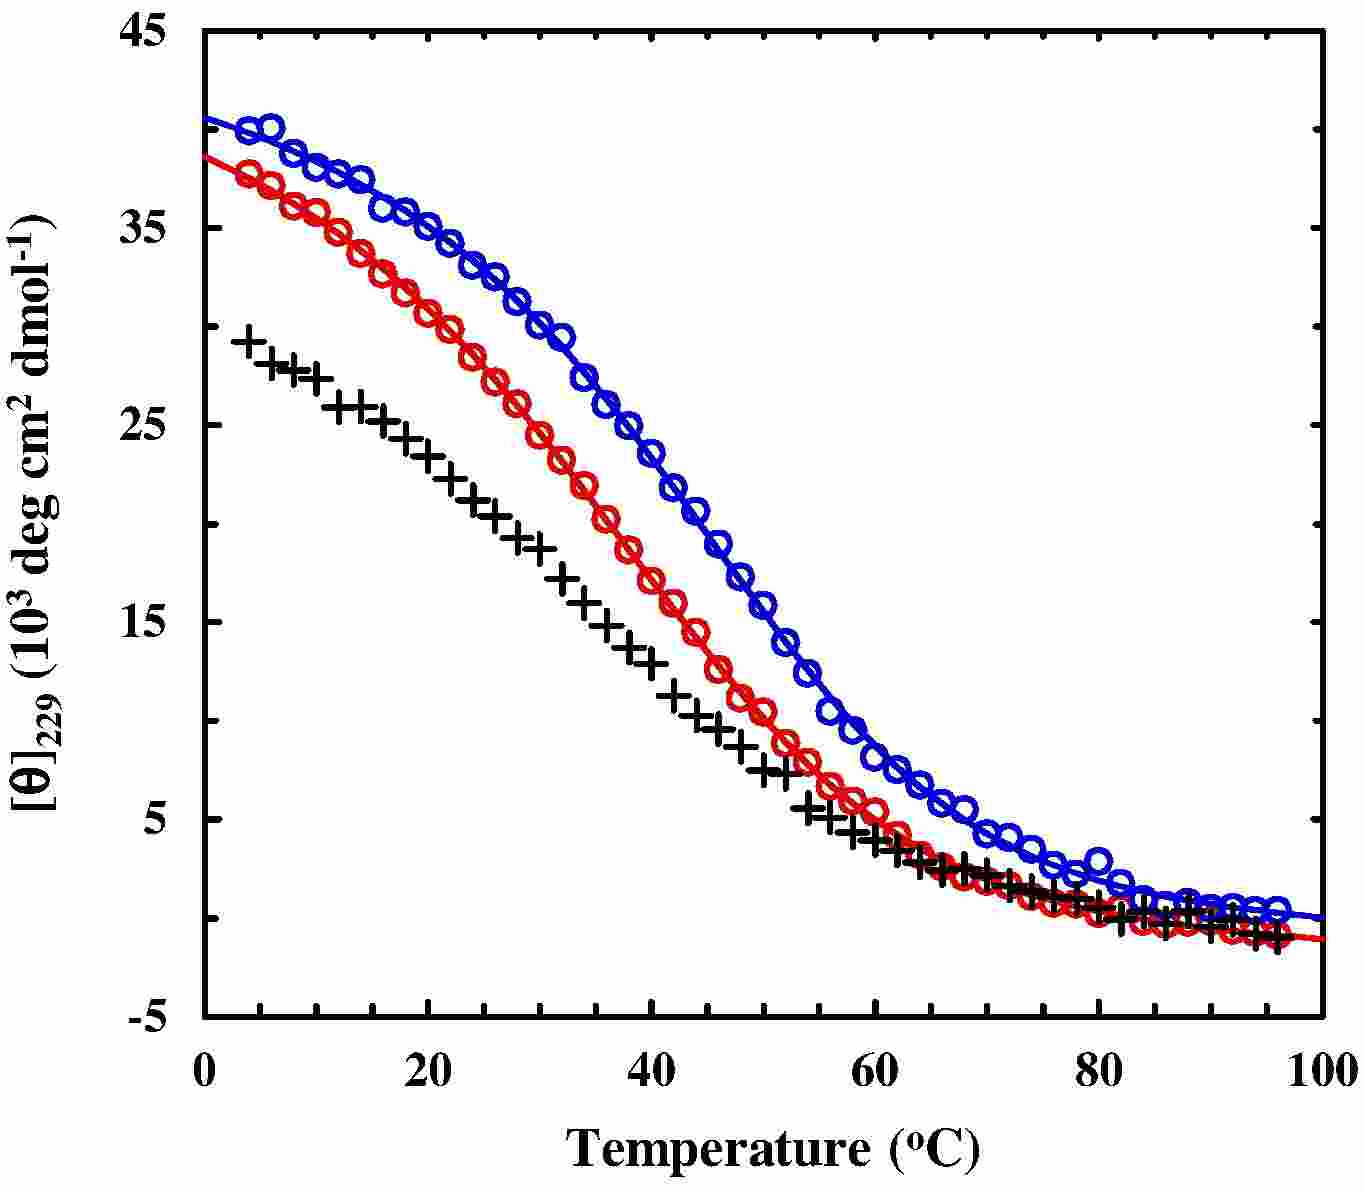
\includegraphics[width=4cm]{pictures/16aa_ff_low.jpg}
\end{center}

\begin{itemize}
\item Isolated $\beta$-sheet experiments are relatively new
\item Comparison between theoretical/experimental studies
\item Detailed thermodynamic MD studies are feasible, but time consuming
\item \bf What effect do crowders have on the folding process?
\end{itemize}

\end{frame}




\section{Monte Carlo Techniques}

\frame{
\frametitle{Monte Carlo: How to sample}
Most methods rely on Monte-Carlo, i.e.\ a selection method that is probabilistically determined. Any method must overcome two obstacles: %\pause
\begin{itemize}[]
\item Enthalpic barriers
\item Entropic barriers (Levinthal's paradox) 
\end{itemize}
%\pause
The enthalpic barriers are usually directly observable from the Hamiltonian while the entropic ones are often more subtle.
}

\frame{
\frametitle{Traditional Sampling Methods}

The typical method uses a Metropolis-Hastings selection scheme:

$$ P(A\rightarrow B) = \exp \left ( \frac{\Delta E_{A,B}}{kT} \right ) $$

%\pause
This works well at finding local minimum - however it needs help getting out. Various models have been designed to get around this such as: Replica Exchange, Simulated Annealing, Reversible Jump Dynamics, etc... \\
\vspace{1em}
%\pause
These simulations only collect data at fixed temperatures; thermodynamic parameters like the free energy or the specific heat at arbitrary temperatures are time consuming
$$
C_V = T \left ( \frac{\partial S}{\partial T} \right ) _ {N,V}
$$
}


\frame{
\frametitle{Wang-Landau}

\begin{itemize}[]
\item Originally designed to solve the Ising model\footnote{F. Wang and D. P. Landau, Phys. Rev. Lett. 86(10), 2001}
\item Extremely effective when the cardinality of $\Omega$ (density of states) is small
\item Can usually be made parallel trivially
\item Works best when energy levels are discrete
\end{itemize}
}

\frame{
\frametitle{Wang-Landau: The equations}
$$ P(A\rightarrow B) = \frac{\Omega(E_A)}{\Omega(E_B)} $$
%\pause
On accepting state:
$$ \Omega(E_{ex}) \rightarrow c \Omega(E_{ex}) $$
%\pause
where $c$ is a constant that is iteratively reduced (originally as):
$$ c \rightarrow \sqrt{c} $$

\vspace{1em}

Once $\Omega(E)$ has converged, we have the partition function \textit{for all temperatures}
$$
Z(T) = \sum \Omega(E_i) \exp ( E_i / kT )
$$

}

\frame{
\frametitle{Wang-Landau}

\begin{itemize}[]
\item Starts as a random walk across the state space 
\item As high entropic states are sampled they become less likely 
\item Random walk $\rightarrow$ biased random-walk 
\item As it converges - detailed balance is obeyed 
\item \textbf{Flat histogram in energy space}
\end{itemize}
}

\section{Modeling and Results}

\begin{frame}
\frametitle{Difficult Questions}
\begin{block}
{How to model?}
\begin{itemize}
\item All-atom? 
\item Explicit water?
\item Effective forces?
\item Level of coarse-graining?
\end{itemize}
\end{block}

\vspace{1em}

We use a face-centered cubic lattice $\Go$-model, with a Potts/Ising approximation for the dihedral angles and aspherical scaled-particle theory to model a crowded solution. 

\vspace{1em}
\textit{lets break that down...} 
\end{frame}


\begin{frame}
\frametitle{Lattice Models\footnote{Chan and Dill, J. Chem. Phys. 118, 8106 (1994)}}

\begin{block}{}
\begin{itemize}
\item Discretize the positions of the amino acids onto a fixed lattice 
\item Short-range interactions dominate (hydrophobicity, charge, etc)
\item Lattice geometry can play a role on the pairing of amino acids
\end{itemize}
\end{block}
\vspace{1em}

\begin{center}
\includegraphics[width=5cm]{../WL_crowding_paper/homopoly_backbone_trim.png}
%\pause
\includegraphics[width=5cm]{../WL_crowding_paper/homopoly_connections_trim.png}
\end{center}
\end{frame}

\begin{frame}
\frametitle{Lattice Choice}
\begin{block}{}
\begin{itemize}
\item High coordination number (FCC vs SC)
\item Common motifs are better represented (alpha, beta)
\item Still a crude approximation to an off-lattice model
\end{itemize}
\end{block}

\begin{block}{}
\begin{center}
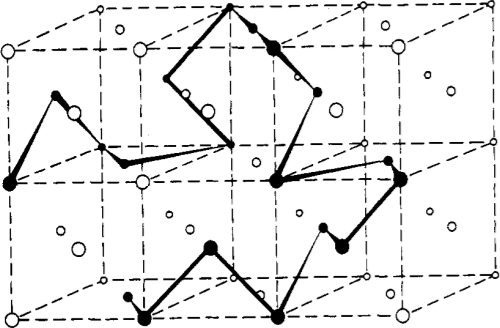
\includegraphics[width=6cm]{pictures/fcc_walk2.png}\\
{\footnotesize Picture from [Downey, 1986]} \\
\end{center}
\end{block}
\end{frame}

\begin{frame}
\frametitle{Ising Model}
\begin{block}{}
\begin{itemize}
\item Analytical solution for 1D (Ising 1925), 2D (Onsager 1944) grids
\item Each vertex on a graph has spin $\sigma \in \{-1, 1\}$, Hamiltonian is the sum over all adjacent spins
$$
\mathcal{H} = -J \sum_{i,j \in \text{edges}} \sigma_i \sigma_j + h \sum_{k \in \text{vertices}} \sigma_k \delta_{1, \sigma_k} 
$$
\item Gives true phase transitions for 2D infinite grids
\item Finite graphs can be solved \textit{exactly}
\end{itemize}
\end{block}
\end{frame}


\frame{
\frametitle{$\Go$-model \& extensions\footnote{\paperrefA}}

\begin{block}{$\Go$-model}
\begin{itemize}
\item Only native-state contacts contribute (all-or-nothing)
\end{itemize}
\end{block}

\begin{block}{Extensions}
\begin{itemize}
\item Extra degree of freedom, each bead now has a `spin'.
\item Accounts for the missing oriental entropy of $\phi-\psi$ angles
\item Only native-state contacts \textit{and} aligned spins contribute, reducing the conformation to a simple graph
\end{itemize}
\end{block}

\begin{center}
\includegraphics[width=5cm]{../WL_crowding_paper/homopoly_connections_trim.png}
\hspace{1em}
\includegraphics[width=5cm]{../WL_crowding_paper/3d_example_graph-crop.pdf}
\end{center}
}


\frame{
\frametitle{General solution to Potts/Ising model {\footnotesize (with external fields!)} }

\begin{block}{With Self-Similarity}
\begin{itemize}
\item Can often be solved/approximated with RG
\item e.g.\ n-dimensional lattices, Cayley/Bethe trees
\end{itemize}
\end{block}

\begin{block}{General Solution}
\begin{itemize}
\item Solved with a subgraph decomposition
\end{itemize}
\end{block}


\begin{figure}[tb]
	\TIKZgraphABC 	\hspace{.5em}
	\TIKZgraphAB	\hspace{.5em}
	\TIKZgraphBC	\hspace{.5em}
	\TIKZgraphC		\hspace{.5em}
\end{figure}


\begin{equation*}
Z = 
\sum_{A \subseteq G} \prod_{c\in C_A}^{k(A)} 
\sum_j^q \paren{ w_j^{n(c)} v_j^{e(c)} } 
\end{equation*}

}

\begin{frame}
\frametitle{Model Hamiltonian}

Hamiltonian counts aligned native contacts in close proximity
\begin{align*}
\mathcal{H}(\mathbf{c},\mathbf{s}) &= -J_+ \KP + J_- \KM  \\ \nonumber
\KP &= \sum_{i=1}^L \sum_{j=i+2}^L \omega_{ij} \mathbf{s}_i \mathbf{s}_j  \GO_{ij} \\ \nonumber
\KM &= \sum_{i=1}^L \sum_{j=i+2}^L \omega_{ij} (1 - \GO_{ij}) 
\end{align*}

Free energy terms for crowding $\Delta \mu$  and entropic cost of alignment $\Delta \psi$
\begin{equation}
\mathcal{F}(\mathbf{c},\mathbf{s}) = \mathcal{H}(\mathbf{c},\mathbf{s})  - \beta \Delta \psi(\sigma) - \beta \Delta \mu(\mathbf{c})
\end{equation}
\end{frame}


\frame{
\frametitle{Fraction Folded\footnote[11]{\paperrefA}}
Measure of fraction folded well-described by model\\

\begin{center}
\begin{figure}[ht]
 \includegraphics[width=8cm]{../WL_crowding_paper/PLOT_all_experimental_fits-crop.pdf}
 %\caption
  \label{fig:Exp_fits}
  \caption{\footnotesize Experimental and modeling data of fraction folded versus temperature. Critical temperatures at $36.1$ and $48.5$ $^\circ$C.}
\end{figure}
\end{center}

}

\frame{
\frametitle{Crowded Conditions\footnote[11]{\paperrefA} 
$\rightarrow$ Folding Stability }
%
\begin{figure}[ht]
 \includegraphics[width=8cm]{../WL_crowding_paper/PLOT_trpzip_CV-crop.pdf}
\caption{\footnotesize Specific heat per residue count for the wild-type peptide trpzip4-m1 in the presence of crowders. Crowders enhance folding stability by shifting melting temperatures by approximately $1.5 ^\circ $C (contrast to experimental value of $12.1 \pm 0.2 ^\circ $C).
}
\end{figure} 
%
}

\frame{
\frametitle{Crowded Conditions \texorpdfstring{$\rightarrow$}{imply} Folding Instability}
While the smaller peptide trpzip4-m1 displays crowding enhanced stability,
the larger designed $\beta$-sheet peptides show (small) instability! \\
\vspace{1em}
\begin{center}
\textbf{Simulations predict that the entropic effect due to the crowding of aspherical proteins may be destabilizing. \\}
\end{center}
\vspace{1em}
%\pause
Why might this be so? \\
\begin{itemize}
\item Ensemble of states has to be considered
\item Only possible with a full density of states calculation
\end{itemize}
}

\frame{
\frametitle{Crowded Conditions \texorpdfstring{$\rightarrow$}{imply} Folding Instability}

Consider the underlying geometry of our $\beta$-sheets\\
\begin{center}
\begin{tabular}{ c c c }
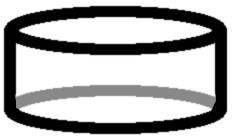
\includegraphics[width=2cm]{pictures/squish_cylin2.jpg} 
 & \hspace{2em} & 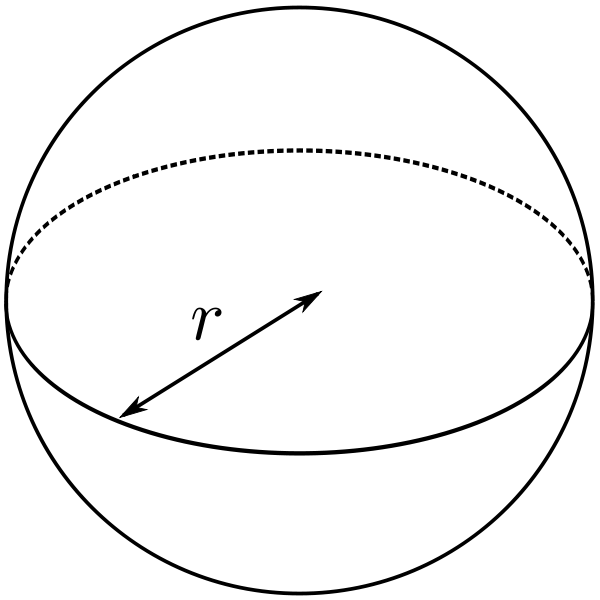
\includegraphics[width=2cm]{pictures/600px-PlainSphere.png} \\
\includegraphics[width=2cm]{../WL_crowding_paper/samplepic1.png} 
	&& \includegraphics[width=2cm]{../WL_crowding_paper/samplepic2.png} 
\end{tabular} \\
{\footnotesize Change of native state conformation under crowding of 3-strand peptide}
\end{center}

\vspace{1em}
\begin{center}
Trade-off between the \textbf{energetically favored native-state}, and an \textbf{entropically unfavorable conformation}.
\end{center}
}


\section{Extensions and Future Work}

\frame{
\frametitle{Macrostate Clustering}

\begin{block}{Group \textbf{micro}states into \textbf{macro}states}
\begin{itemize}
\item Coarse-grain from kinetics, compute transition probabilities
\item Transpose of eigenvectors suggest clustering
\end{itemize}
\end{block}

\begin{block}{Example: Random walk in a three-well potential}
\includegraphics[height=.3\textwidth]{../supplement/smooth_potential_cluster/pictures/smooth_potential_traj.png}
\includegraphics[height=.3\textwidth]{../supplement/smooth_potential_cluster/pictures/cluster_locations.png}
\end{block}




}

\frame{
\frametitle{Future Work}

Where is the field going? \\
What are the important questions? \\
\vspace{1em}

\begin{block}
{Nuanced Interactions}
\begin{itemize}
\item Electrostatic Effects
\item Hydrophobicity
\item Hydrogen Bonds
\end{itemize}
\end{block}
\vspace{1em}

%\pause

\begin{block}
{Beyond thermodynamics}
\begin{itemize}
\item Protein function and activity
\item Aggregation models and kinetics
\item Diffusion rates in crowded environments
\end{itemize}
\end{block}
}

\frame{
\thispagestyle{empty}
\addtocounter{framenumber}{-1} 
\begin{center}

\includegraphics[width=.8\textwidth]{pictures/thankyou.pdf} 
\end{center}
}

\appendix

\frame{
\frametitle{Extra: Scaled Particle Theory Equations}

\thispagestyle{empty}
\addtocounter{framenumber}{-1} 

\begin{block}{Activity coefficient}
\vspace{-1em}
\begin{equation*}
\textstyle
\ln{\gamma_i} = -\ln(1-\paren{V}) 
+ \frac{H_i \paren{S} + S_i\paren{H} + V_i\paren{1}}{1-\paren{V}} 
+ \frac{H_i^2 \paren{S}^2 + 2 V_i \paren{H}\paren{S}}{2(1-\paren{V})^2}
+ \frac{V_i \paren{H^2}\paren{S}^2 }{3(1-\paren{V})^3}
\end{equation*}
\end{block}

$H$ is the Kihara support function, geometrical measure of `roundness' \\


For example: \\
\begin{center}
\begin{tabular}{ l c c }
$H_\text{\text{sphereocylin}} = r\pi/4 + L/2$ & \hspace{4em} & 
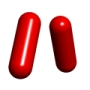
\includegraphics[height=1cm]{pictures/sphereocylinder.jpg} \\
$H_{\text{cylinder}} = r + L/4$ &&
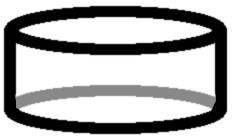
\includegraphics[height=1cm]{pictures/squish_cylin2.jpg} \\
\end{tabular}
\end{center}
\vspace{1em}
We model the crowders, Ficoll 70, as sphereocylinders
\footnote{Fodeke and Minton, J. Phys. Chem. B 114, 10876 (2010)} and the $\beta$-sheet peptides as cylinders to best match their native state geometry.
}


% End of slides
\end{document}